% Standalone entry point. Compile this file or upload this directory to Overleaf.
\documentclass[11pt]{article}
\usepackage[margin=1in]{geometry}
\usepackage[T1]{fontenc}
\usepackage{lmodern}
\usepackage{amsmath,amssymb,mathtools}
\usepackage{booktabs,tabularx,longtable,array}
\usepackage{graphicx,microtype}
\usepackage{enumitem}
\usepackage[numbers,sort&compress]{natbib}
\usepackage{xcolor}
\usepackage{tikz}
\usetikzlibrary{arrows.meta,positioning,calc}
\usepackage[colorlinks=true,linkcolor=blue!55!black,citecolor=blue!55!black,urlcolor=blue!55!black]{hyperref}
% Prefixed commands minimize collisions with an existing manuscript.
\providecommand{\methodname}{V4}
\providecommand{\vfourBio}{V4+Bio}
\providecommand{\vunit}[1]{\operatorname{n}(#1)}
\providecommand{\vLN}{\operatorname{LN}}
\providecommand{\vGELU}{\operatorname{GELU}}
\providecommand{\vReLU}{\operatorname{ReLU}}
\providecommand{\vDrop}{\operatorname{Drop}_{0.1}}
\providecommand{\vsoftmax}{\operatorname{softmax}}
\providecommand{\vsigmoid}{\operatorname{sigmoid}}
\providecommand{\vpos}[1]{\left[#1\right]_{+}}
\providecommand{\vR}{\mathcal{R}_{\mathrm{tr}}}
\providecommand{\vE}{\mathcal{E}_{\mathrm{tr}}}
\providecommand{\vD}{\mathcal{D}_{\mathrm{tr}}}
\providecommand{\vFamilies}{\{\mathrm{EC},\mathrm{cof},\mathrm{mech}\}}

\setlength{\emergencystretch}{2em}
\allowdisplaybreaks
\title{\methodname: Architecture, Training Objectives, and Retrieval\\\large Detailed methods draft}
\author{}
\date{Implementation snapshot: 21 September 2026}
\begin{document}
\maketitle
\begin{abstract}
We describe a bidirectional enzyme--reaction retrieval method with independently
computable protein and reaction representations. The protein encoder combines a
global sequence representation, a frozen SLEEC residue prior, and four learned
residue views. The reaction encoder combines frozen reaction, molecular, and
chemical features. Training comprises minibatch, anchor-balanced multi-positive
alignment followed by full-graph residual refinement. The final retrieval score
combines the refined neural representation with a fixed dictionary of training
reactions. An optional biological objective regularizes the existing refinement
heads using EC hierarchy, cofactor-associated categories, and coarse
transformation descriptors, without introducing additional inference parameters.
This document specifies the original V4 recipe and its phase-2-only biological
variant, including the exact distinction between their training and inference
computations.
\end{abstract}
\tableofcontents
\clearpage
% Main methods fragment. Requires macros.tex and the packages in main.tex.
% This is the implemented V4 / phase-2-only all_1 recipe, not a proposed model.
\section{Method}
\label{sec:v4-method}

\subsection{Problem formulation and overview}
\label{sec:v4-problem}
Let $\vR=\{r_1,\ldots,r_{N_R}\}$ and
$\vE=\{e_1,\ldots,e_{N_E}\}$ denote the unique reaction and enzyme
identifiers appearing in a target dataset's training split. The observed
association graph is $\vD\subseteq\vR\times\vE$, with binary adjacency
$Y_{ij}=\mathbb{1}[(r_i,e_j)\in\vD]$. A reaction can have several associated
enzymes and an enzyme can have several associated reactions. We learn a score
$S(r,e)$ used to rank enzymes for a reaction ($R\!\to\!E$) or reactions for an
enzyme ($E\!\to\!R$). The score is a retrieval compatibility measure, rather
than a calibrated probability of catalytic activity.

\methodname has independent protein and reaction encoders. Phase 1 learns
512-dimensional neural representations from the target training associations.
Phase 2 freezes these encoders and learns a small residual refinement for each
endpoint using the complete target training graph. At inference, the refined
representations are combined with a fixed representation whose coordinates
index training reactions (Figure~\ref{fig:v4-architecture}). Candidate vectors
can therefore be precomputed: encoding a protein does not require the current
reaction query, and encoding a reaction does not require the current screening
library.

We describe two objectives for the same architecture. Original \methodname
uses association supervision and geometry preservation in phase 2.
\vfourBio adds a relative biological neighborhood loss to those same heads.
For the reported \texttt{all\_1} configuration, biological supervision is used
only in phase 2. The protein residue queries, SLEEC scorer, reaction encoder,
and dictionary remain fixed during this addition.

Throughout, $\vunit{x}=x/\max(\lVert x\rVert_2,\epsilon)$ denotes numerical
$\ell_2$ normalization, $\vpos{x}=\max(0,x)$, $[x;y]$ denotes concatenation,
and $\vLN$ denotes layer normalization. All attention distributions exclude
padding. Distinct occurrences of a learnable projection have independent
parameters unless sharing is explicitly stated.

\begin{figure}[tb]
\centering
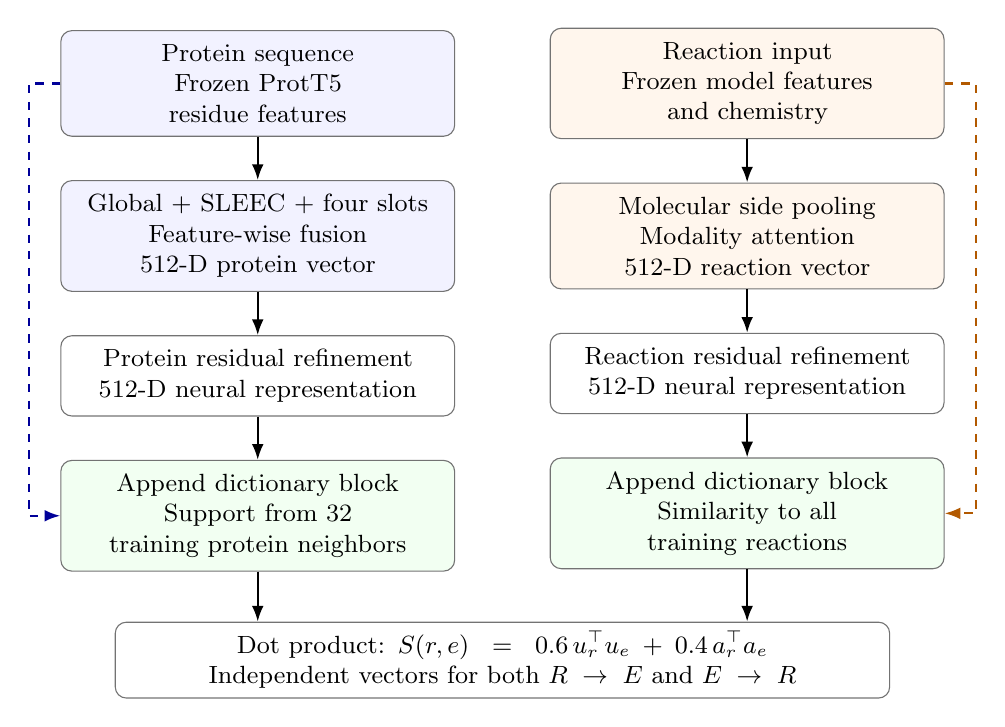
\begin{tikzpicture}[
    box/.style={draw=black!55,rounded corners,align=center,font=\small,
                text width=4.65cm,minimum height=1.0cm,inner sep=5pt},
    arrow/.style={-{Latex[length=2mm]},thick},node distance=0.55cm]
  \node[box,fill=blue!5] (protein) {Protein sequence\\Frozen ProtT5\\residue features};
  \node[box,fill=orange!7,right=1.2cm of protein] (reaction) {Reaction input\\Frozen model features\\and chemistry};
  \node[box,fill=blue!5,below=of protein] (pe) {Global + SLEEC + four slots\\Feature-wise fusion\\512-D protein vector};
  \node[box,fill=orange!7,below=of reaction] (re) {Molecular side pooling\\Modality attention\\512-D reaction vector};
  \node[box,below=of pe] (ph) {Protein residual refinement\\512-D neural representation};
  \node[box,below=of re] (rh) {Reaction residual refinement\\512-D neural representation};
  \node[box,fill=green!5,below=of ph] (pa) {Append dictionary block\\Support from 32\\training protein neighbors};
  \node[box,fill=green!5,below=of rh] (ra) {Append dictionary block\\Similarity to all\\training reactions};
  \node[draw=black!55,rounded corners,align=center,font=\small,
        text width=9.6cm,below=0.65cm of $(pa.south)!0.5!(ra.south)$] (score)
       {Dot product: $S(r,e)=0.6\,u_r^\top u_e+0.4\,a_r^\top a_e$\\
        Independent vectors for both $R\!\to\!E$ and $E\!\to\!R$};
  \draw[arrow] (protein)--(pe); \draw[arrow] (reaction)--(re);
  \draw[arrow] (pe)--(ph); \draw[arrow] (re)--(rh);
  \draw[arrow] (ph)--(pa); \draw[arrow] (rh)--(ra);
  \draw[arrow,dashed,draw=blue!60!black] (protein.west) -- ++(-0.4,0) |- (pa.west);
  \draw[arrow,dashed,draw=orange!70!black] (reaction.east) -- ++(0.4,0) |- (ra.east);
  \draw[arrow] (pa.south)--(score.north -| pa.south);
  \draw[arrow] (ra.south)--(score.north -| ra.south);
\end{tikzpicture}
\caption{Inference structure of \methodname. Dashed paths supply frozen raw
features to the dictionary maps. Dictionary coordinates are computed
from frozen raw features and training associations, independently of the neural
refinement heads. The arrows into the appended representations indicate
composition, not that dictionary features are generated from the heads.
The optional biological loss acts on the two residual heads during phase 2;
it introduces no additional inference branch. The protein fused-view multiplier
and refinement multiplier are specified in Section~\ref{sec:v4-inference}.}
\label{fig:v4-architecture}
\end{figure}


\subsection{Protein encoder: global, SLEEC, and learned residue views}
\label{sec:v4-protein}
For an enzyme sequence $e$ with $L$ retained residues, a frozen ProtT5 model
provides contextual residue vectors
$H_e=[h_1,\ldots,h_L]^\top\in\mathbb{R}^{L\times1024}$
\citep{elnaggar2022prottrans}. We construct six protein views: one global
view, one view defined by a frozen SLEEC functional-residue scorer
\citep{gong2026sleec}, and $K=4$ learned residue views. The scorer is a
pretrained resource; it is not fitted to each retrieval target in phase 1.

\paragraph{Global and SLEEC views.}
The global view is the mean of the retained residue embeddings,
\begin{equation}
  x^{(0)}_e=\frac{1}{L}\sum_{i=1}^{L}h_i.
  \label{eq:v4-global}
\end{equation}
The frozen scorer computes a scalar logit $\ell_i$ for each residue using a
$1024\!\to\!256\!\to\!1$ MLP with a ReLU hidden activation. We center these
logits within the protein, clip them, and form a smoothed attention distribution:
\begin{align}
  \bar\ell &= L^{-1}\sum_{i=1}^{L}\ell_i,
  & t_i &= \operatorname{clip}(\ell_i-\bar\ell,-10,10),\\
  p_i^{\mathrm{S}} &= \frac{\exp(t_i)}{\sum_{j=1}^{L}\exp(t_j)},
  & a_i^{\mathrm{S}} &= (1-\eta)p_i^{\mathrm{S}}+\frac{\eta}{L},
  \quad \eta=0.05,\\
  x_e^{(1)} &= \sum_{i=1}^{L}a_i^{\mathrm{S}}h_i.
  \label{eq:v4-sleec}
\end{align}
Thus, SLEEC contributes a soft residue-weighted view. The threshold used for
SLEEC diagnostics does not select or remove residues in this encoder.

\paragraph{Four learned residue views.}
A shared residue adapter maps each contextual residue to $d_h=256$ dimensions:
\begin{equation}
  \tilde h_i=\vGELU(W_a\vLN(h_i)+b_a),\qquad
  k_i=\vunit{W_k\tilde h_i},\qquad
  v_i=W_v\tilde h_i+b_v.
  \label{eq:v4-residue-adapter}
\end{equation}
Here $W_k$ has no bias. The model contains four shared trainable query vectors
$q_k\in\mathbb{R}^{256}$, initialized orthogonally. They are model parameters,
not reaction-dependent queries. For slot $k$, attention is
\begin{align}
  \gamma &=10\vsigmoid(\rho_\gamma),\qquad \gamma_{\mathrm{init}}=4,\\
  p_{ki}&=\frac{\exp\!\left(\gamma\,\vunit{q_k}^{\top}k_i\right)}
                     {\sum_{j=1}^{L}\exp\!\left(\gamma\,\vunit{q_k}^{\top}k_j\right)},
  & a_{ki}&=(1-\eta)p_{ki}+\frac{\eta}{L},\\
  x_e^{(k+1)}&=\sum_{i=1}^{L}a_{ki}v_i,
  & k&\in\{1,\ldots,4\}.
  \label{eq:v4-slots}
\end{align}
Each slot can select a different content-dependent summary of the same
protein. The four views are fused into one protein vector; they are not four
independently scored enzyme prototypes. SLEEC defines its own view and is not
added as a common logit bias to the four learned slots.

\paragraph{Feature-wise view fusion.}
Each view is projected to 256 dimensions by an independent network
\begin{equation}
  F_{a\to b}(x)=W_2\vDrop\!\left(\vGELU(W_1\vLN(x)+b_1)\right)+b_2,
  \label{eq:v4-protein-ffn}
\end{equation}
whose hidden width is 512 and whose training dropout probability is 0.1.
For the first two views $a=1024$; for learned slots $a=256$. Define
$y_e^{(v)}=\vunit{F_v(x_e^{(v)})}$ for $v=0,\ldots,5$.
A $1536\!\to\!256\!\to\!1536$ gate MLP with GELU maps their concatenation
to logits $G_e\in\mathbb{R}^{6\times256}$. The gate softmax is taken over
views \emph{separately for each feature coordinate}:
\begin{align}
  \omega_{vj}
    &=(1-\zeta)\frac{\exp(G_{vj})}{\sum_{u=0}^{5}\exp(G_{uj})}
       +\frac{\zeta}{6},\qquad \zeta=0.05,\\
  \bar y_{e,j}&=\sum_{v=0}^{5}\omega_{vj}\,y_{e,j}^{(v)}.
  \label{eq:v4-view-gate}
\end{align}
The final gate layer is initialized to zero, giving equal initial view
weights. The floor is $\zeta/6$ per view and coordinate, not 0.05 per view.

Two additional networks of the form in Eq.~\eqref{eq:v4-protein-ffn} produce
separately normalized global and fused outputs in $\mathbb{R}^{512}$:
\begin{align}
  g_e &= \vunit{F_g(x_e^{(0)})}, & f_e&=\vunit{F_f(\bar y_e)},\\
  s&=0.5\vsigmoid(\rho_s), & b_e&=\vunit{g_e+s f_e}.
  \label{eq:v4-protein-output}
\end{align}
The scalar $s$ is shared across proteins, is initialized to 0.1, and remains
strictly between 0 and 0.5. The direct global branch provides a stable route
from the mean sequence features while the fused branch learns a correction.

\paragraph{Sequence order and interpretation.}
No additional positional encoding is applied in the pooling module. Its
queries attend to the contextual content of ProtT5 vectors. Permuting already
computed residue vectors and their masks together leaves this pooling operation
unchanged, whereas changing the amino-acid sequence can change the contextual
vectors. Neither a slot nor a coordinate of the final 512-dimensional vector
is assigned a named catalytic function. Attention weights are learned
aggregation weights, not validated active-site labels.

\subsection{Reaction encoder: molecular sides and modality fusion}
\label{sec:v4-reaction}
We use four feature sources: a 768-dimensional ReactionT5v2 reaction embedding
\citep{sagawa2023reactiont5,sagawaReactionT5v2}, 768-dimensional Uni-Mol2
molecule embeddings \citep{ji2024unimol2}, 256-dimensional ChIRo molecule
embeddings \citep{adams2022chiro}, and a 617-dimensional fixed chemistry
vector. Their feature extractors are frozen; molecular pooling, modality
projections, and fusion are trainable.

\paragraph{Side-specific molecule pooling.}
For molecular modality $m\in\{\mathrm{UniMol2},\mathrm{ChIRo}\}$ and side
$s\in\{-,+\}$, let $x_{s,j}^{m}$ be the embedding of molecule $j$.
Independent linear attention scorers for the two sides produce
\begin{equation}
  \pi_{s,j}^{m}=
    \frac{\exp((w_s^m)^\top x_{s,j}^{m}+b_s^m)}
         {\sum_t\exp((w_s^m)^\top x_{s,t}^{m}+b_s^m)},
  \qquad
  p_s^m=\sum_j\pi_{s,j}^{m}x_{s,j}^{m}.
  \label{eq:v4-molecule-pool}
\end{equation}
The configured \texttt{directional\_delta} composition is
\begin{equation}
  c_r^m=[p_-^m;\ p_+^m;\ p_+^m-p_-^m;\ |p_+^m-p_-^m|].
  \label{eq:v4-directional}
\end{equation}
It has dimension 3072 for Uni-Mol2 and 1024 for ChIRo. Direction is represented
by the ordered sides and signed difference when physical sides are supplied.

\paragraph{Input semantics.}
For EnzymeMap, inputs retain their physical reactant and product sides.
ReactZyme's released participant-set inputs use the established self-reaction
adapter, placing the same complete set on both sides. The two side poolers
still have different parameters, so their pooled vectors need not be equal.
Their difference on these self-reactions must not be interpreted as an
observed chemical transformation direction. The choice of chemical input
representation is separate from the choice of retrieval direction.

\paragraph{Modality tokens and attention.}
For $m\in\{\mathrm{T5},\mathrm{UniMol2},\mathrm{ChIRo},\mathrm{chem}\}$,
let $c_r^m$ denote the corresponding reaction input. Each independent modality
MLP has widths $d_m\!\to\!1024\!\to\!512\!\to\!512$, with ReLU after
the first two linear layers. A shared layer-normalization module then gives
the modality token
\begin{equation}
  t_r^m=\vLN(\operatorname{MLP}_m(c_r^m))\in\mathbb{R}^{512}.
\end{equation}
An attention MLP of widths $512\!\to\!512\!\to\!1$, with a ReLU hidden
activation, scores the tokens. If $\mathcal M_r$ is the set of available
modalities,
\begin{equation}
  \alpha_r^m=
  \frac{\exp(A(t_r^m))}{\sum_{n\in\mathcal M_r}\exp(A(t_r^n))},
  \quad
  t_r=\sum_{m\in\mathcal M_r}\alpha_r^m t_r^m,
  \quad
  b_r=\vunit{F_r(t_r)}.
  \label{eq:v4-reaction-output}
\end{equation}
The output MLP $F_r$ has widths $512\!\to\!1024\!\to\!512$ and a ReLU
hidden activation. Unavailable modalities are masked out of attention.
Reaction modality dropout and projection dropout are zero in the reported
recipe. The resulting $b_r$ and $b_e$ inhabit a shared 512-dimensional
retrieval space.

\subsection{Phase 1: anchor-balanced, decoupled multi-positive alignment}
\label{sec:v4-phase1}
Training minibatches sample association rows and deduplicate their endpoint
identifiers before constructing a reaction-by-enzyme score matrix. Let
$\mathcal R_B$ and $\mathcal E_B$ be these distinct endpoints. Positives are
identified from \emph{all known training associations between endpoints in
the batch}, rather than only the association rows sampled for that batch.
For a reaction anchor $r$, define
\begin{equation}
  P_B(r)=\{e\in\mathcal E_B:(r,e)\in\vD\},\qquad
  N_B(r)=\mathcal E_B\setminus P_B(r),
\end{equation}
and define $P_B(e)$ and $N_B(e)$ analogously for enzyme anchors. Only anchors
with at least one positive and one remaining candidate enter the respective
directional average.

The logits are $z_{re}=\beta b_r^\top b_e$ with fixed inverse temperature
$\beta=5$ (temperature 0.2). For each known positive $p$ of an anchor $a$, the
decoupled loss is
\begin{align}
  \ell_{\mathrm{dec}}(a,p)
   &=-\log\frac{\exp(z_{ap})}
       {\exp(z_{ap})+\sum_{n\in N_B(a)}\exp(z_{an})}\\
   &=\log\left(1+\sum_{n\in N_B(a)}\exp(z_{an}-z_{ap})\right).
   \label{eq:v4-decoupled}
\end{align}
Other known positives are excluded from the denominator for this individual
positive. Thus every positive must compete with the remaining candidates,
without competing with its known positive partners. This differs from a
single log-sum over all positives, which can be dominated by one easy positive.

Let $\mathcal A_R$ and $\mathcal A_E$ be the valid reaction and enzyme anchors
in the batch. We first average over positives within an anchor, then average
over anchors, and finally average the two directions:
\begin{align}
  \mathcal L_{R\to E}^{(1)}
    &=\frac{1}{|\mathcal A_R|}\sum_{r\in\mathcal A_R}
      \frac{1}{|P_B(r)|}\sum_{e\in P_B(r)}\ell_{\mathrm{dec}}(r,e),\\
  \mathcal L_{E\to R}^{(1)}
    &=\frac{1}{|\mathcal A_E|}\sum_{e\in\mathcal A_E}
      \frac{1}{|P_B(e)|}\sum_{r\in P_B(e)}\ell_{\mathrm{dec}}(e,r),\\
  \mathcal L_{\mathrm{align}}^{(1)}
    &=\tfrac12\mathcal L_{R\to E}^{(1)}+
      \tfrac12\mathcal L_{E\to R}^{(1)}.
  \label{eq:v4-anchor-balanced}
\end{align}
A direction with no valid anchor contributes zero. The normalization prevents
an anchor's contribution from growing simply in proportion to its number of
positives in the matrix. It does not make anchors equally frequent over an
epoch when association rows are sampled. Unobserved pairs are still used as
contrastive negatives with weight 1; they are not measured inactive pairs.

\paragraph{Attention regularization.}
The protein encoder also returns two small penalties on the \emph{raw}
learned-slot distributions $p_{ki}$, before the uniform mixture in
Eq.~\eqref{eq:v4-slots}. For a protein of length $L$, define
\begin{align}
  H_k&=-\sum_i p_{ki}\log p_{ki},\qquad
  H_{\min}(L)=\min\{\tfrac12\log L,\log4\},\\
  E(e)&=\frac1K\sum_{k=1}^{K}\vpos{H_{\min}(L)-H_k}^{2}.
  \label{eq:v4-entropy}
\end{align}
This penalty discourages attention with very small effective support. To
discourage nearly identical attention patterns, center each raw distribution
against uniform attention: $\bar p_k=p_k-L^{-1}\mathbf 1$. For eligible
unordered pairs $\mathcal Q_e=\{(k,l):k<l,\ \|\bar p_k\|_2>10^{-6},
\ \|\bar p_l\|_2>10^{-6},\ L>1\}$, let
\begin{equation}
  D(e)=\frac{1}{\max(1,|\mathcal Q_e|)}
     \sum_{(k,l)\in\mathcal Q_e}
       \vpos{\frac{\bar p_k^\top\bar p_l}
                         {\|\bar p_k\|_2\|\bar p_l\|_2}-0.9}^{2}.
  \label{eq:v4-diversity}
\end{equation}
Uniform heads have no meaningful centered direction and are excluded from
this comparison. The complete phase-1 objective is
\begin{equation}
  \boxed{\mathcal L^{(1)}=
      \mathcal L_{\mathrm{align}}^{(1)}
      +0.01\,\frac{1}{|\mathcal E_B|}\sum_{e\in\mathcal E_B}E(e)
      +0.01\,\frac{1}{|\mathcal E_B|}\sum_{e\in\mathcal E_B}D(e).}
  \label{eq:v4-phase1-total}
\end{equation}
There is no EC/cofactor/mechanism loss in this phase for the phase-2-only
\vfourBio configuration. The safeguards in Eqs.~\eqref{eq:v4-entropy}
and~\eqref{eq:v4-diversity} encourage numerical and representational diversity;
they do not establish a biological interpretation of the attention heads.

\subsection{Phase 2: full-graph residual refinement}
\label{sec:v4-phase2}
After selecting the epoch-10 phase-1 snapshot, we freeze both F3 encoders and
cache their unadjusted outputs $b_r,b_e$ for the unique training endpoints.
Two independent residual heads $h_R,h_E$ each comprise layer normalization,
a $512\!\to\!1024$ linear layer, GELU, and a $1024\!\to\!512$ linear
layer. The last layer's weights and biases are initialized to zero. During
phase-2 training,
\begin{equation}
  u_r^{\mathrm{tr}}=\vunit{b_r+\kappa h_R(b_r)},\qquad
  u_e^{\mathrm{tr}}=\vunit{b_e+\kappa h_E(b_e)},\qquad \kappa=0.2.
  \label{eq:v4-residual-training}
\end{equation}
Consequently, both heads initially preserve the normalized base
representations. No gradient is propagated to the frozen F3 encoders.

\paragraph{Uniform-positive cross-entropy over the complete graph.}
We form the full training matrix $Z_{ij}=(u_{r_i}^{\mathrm{tr}})^\top
u_{e_j}^{\mathrm{tr}}/\tau_2$, with $\tau_2=0.2$. Let
$d_i^R=\sum_jY_{ij}$ and $d_j^E=\sum_iY_{ij}$. Every retained training
endpoint has at least one association. The directional objectives are
\begin{align}
  \mathcal L_{R\to E}^{(2)}
    &=\frac{1}{N_R}\sum_i\left[
       \log\sum_{j=1}^{N_E}\exp(Z_{ij})
       -\frac{1}{d_i^R}\sum_jY_{ij}Z_{ij}\right],\\
  \mathcal L_{E\to R}^{(2)}
    &=\frac{1}{N_E}\sum_j\left[
       \log\sum_{i=1}^{N_R}\exp(Z_{ij})
       -\frac{1}{d_j^E}\sum_iY_{ij}Z_{ij}\right],\\
  \mathcal L_{\mathrm{CE}}^{(2)}
    &=\tfrac12\mathcal L_{R\to E}^{(2)}+
      \tfrac12\mathcal L_{E\to R}^{(2)}.
  \label{eq:v4-fullgraph}
\end{align}
These are cross-entropies with a uniform target distribution over each
anchor's known positives. Unlike phase 1, the denominator includes all
opposite-type training endpoints, including all positives. Phase 2 therefore
changes both the coverage of the contrastive bank and the form of the loss;
it is not simply Eq.~\eqref{eq:v4-decoupled} evaluated on a larger batch.

\paragraph{Preserving the original geometry.}
An identity penalty limits changes to the frozen base representations:
\begin{equation}
  \mathcal L_{\mathrm{id}}=
  \frac{1}{2N_R}\sum_i\left[1-(u_{r_i}^{\mathrm{tr}})^\top\vunit{b_{r_i}}\right]
  +\frac{1}{2N_E}\sum_j\left[1-(u_{e_j}^{\mathrm{tr}})^\top\vunit{b_{e_j}}\right].
  \label{eq:v4-identity}
\end{equation}
The original \methodname phase-2 objective is
$\mathcal L_{\mathrm{CE}}^{(2)}+10\mathcal L_{\mathrm{id}}$.
Both heads are optimized jointly for 100 updates, each of which includes the
entire compact training graph.

\subsection{Biological supervision without additional encoder components}
\label{sec:v4-biology}
The biological extension modifies the training objective of these same heads.
It constrains relationships among reaction representations and, separately,
among enzyme representations. The association loss connects the two endpoint
types. No classification heads, biological feature coordinates, additional
residue queries, or inference-time annotation inputs are introduced.

\paragraph{Annotation families and confidence.}
We use three families $\mathcal F=\vFamilies$. Each training endpoint can
belong to multiple categories. A membership in category $c$ has confidence
$w_{ic}\in(0,1]$; missing memberships create no annotation evidence.
For EC, each specified prefix is retained. A category at hierarchy depth
$d\in\{1,2,3,4\}$ has weight
$\xi_c\in\{0.125,0.25,0.5,1\}$, respectively. Unknown EC digits are not
imputed. Cofactor-associated categories are recognized from reaction
participants and assigned confidence 0.4. They describe participant presence,
which is an imperfect proxy for a biochemical cofactor requirement.
Mechanism categories are coarse descriptors derived from atom-mapped bond
changes; mappings below confidence 0.5 are omitted. These descriptors do not
specify complete catalytic mechanisms. Cofactor and mechanism category
weights are $\xi_c=1$.

Reaction annotations are transferred to proteins only along training
associations. When several observations support the same membership, the
maximum confidence is retained. Native protein EC annotations can additionally
describe multiple functions of a training protein. Appendix~\ref{app:v4-annotations}
specifies the different annotation sources for the two benchmarks.

\paragraph{Relative within-category and background distances.}
Consider one endpoint type $X\in\{R,E\}$ and one family $f$. Let
$\hat z_i=\vunit{u_i^{\mathrm{tr}}}$ and
$\delta_{ij}=1-\hat z_i^\top\hat z_j$.
Let $I_c$ be the endpoints annotated with category $c$, $n_c=|I_c|$, and
$\mathcal A_f=\bigcup_{c\in f}I_c$. The comparison set is
$B_c=\mathcal A_f\setminus I_c$. An endpoint without any annotation in $f$
is excluded from both membership and background for that family. For a
multiply annotated background endpoint, set
$\bar w_j^f=\max_{c'\in f:j\in I_{c'}}w_{jc'}$.

For eligible categories, define the within-category and background confidence
masses
\begin{equation}
  T_c=\sum_{\substack{i,j\in I_c\\i\ne j}}w_{ic}w_{jc},\qquad
  U_c=\sum_{i\in I_c}\sum_{j\in B_c}w_{ic}\bar w_j^f,
\end{equation}
and confidence-weighted mean distances
\begin{align}
  d_c^{\mathrm{within}}
    &=\frac{1}{T_c}
       \sum_{\substack{i,j\in I_c\\i\ne j}}w_{ic}w_{jc}\delta_{ij},\\
  d_c^{\mathrm{background}}
    &=\frac{1}{U_c}\sum_{i\in I_c}\sum_{j\in B_c}
          w_{ic}\bar w_j^f\delta_{ij}.
  \label{eq:v4-bio-distances}
\end{align}
The per-category penalty is
\begin{equation}
  \ell_c=\underbrace{\frac{T_c}{n_c(n_c-1)}}_{\text{mean pair confidence}}
       \vpos{m+d_c^{\mathrm{within}}-d_c^{\mathrm{background}}},
       \qquad m=0.1.
  \label{eq:v4-relative-bio}
\end{equation}
Its prefactor preserves the strength of annotation confidence. For example,
if every membership in a category has confidence 0.4, this prefactor is
$0.4^2=0.16$. Computing only confidence-normalized distances would remove
that common confidence reduction.

A category contributes only if $n_c\ge2$, $|B_c|\ge1$, $T_c>0$, and
$U_c>0$. Let $\mathcal C_{X,f}^{*}$ be the eligible categories. We use a
category-weighted average, followed by a fixed average over endpoint types:
\begin{equation}
  \mathcal L_{X,f}=
    \frac{\sum_{c\in\mathcal C_{X,f}^{*}}\xi_c\ell_c}
         {\sum_{c\in\mathcal C_{X,f}^{*}}\xi_c},\qquad
  \mathcal L_f=\tfrac12(\mathcal L_{R,f}+\mathcal L_{E,f}).
  \label{eq:v4-family-average}
\end{equation}
An empty eligible set contributes zero. Averaging by category, rather than
by the total number of pairs across categories, limits domination by very
large annotation groups. Membership overlap is allowed; the background for
one category can share other categories with its members.

\paragraph{Complete biological phase-2 objective.}
For \vfourBio, the exact objective is
\begin{equation}
  \boxed{\mathcal L^{(2)}=
     \mathcal L_{\mathrm{CE}}^{(2)}+10\mathcal L_{\mathrm{id}}
     +\frac13\sum_{f\in\mathcal F}\lambda_f\mathcal L_f.}
  \label{eq:v4-phase2-total}
\end{equation}
The \texttt{all\_1} configuration sets all three $\lambda_f=1$; original
\methodname sets all three to zero. In family-removal controls, only the
corresponding coefficient is set to zero; the divisor remains three.
Shuffled-label controls preserve annotation profiles, confidences, and
category frequencies while permuting their assignment to training endpoints.

The relative loss expresses a geometric preference for annotated peers. The
background does not assert that a protein is inactive for a reaction, and
different categories are not mutually exclusive biological functions.
Incomplete annotations and enzyme promiscuity can make these geometric
references imperfect. The relative hinge does not by itself guarantee
non-collapsed embeddings; association supervision remains necessary. In the
phase-2-only variant, biological gradients reach the residual heads but not
the frozen residue queries or feature extractors. Exact category-sum
identities avoid constructing a dense biological pairwise matrix
(Appendix~\ref{app:v4-efficient-bio}).

\subsection{Training-reaction dictionary representation}
\label{sec:v4-dictionary}
In addition to the neural embedding, both endpoints receive a vector
$a\in\mathbb{R}^{N_R}$ whose coordinates index the target's training
reactions. The dictionary uses frozen raw features and observed training
associations. It is fitted once for each target split and is independent of
the current query or candidate collection.

\paragraph{Training-only centering.}
For a raw feature family with available training values $x_i$, we compute
\begin{equation}
  \mu=\frac{1}{N_{\mathrm{avail}}}\sum_{i\in\mathrm{available\ train}}\vunit{x_i},
  \qquad \psi(x)=\vunit{\vunit{x}-\mu}.
  \label{eq:v4-center}
\end{equation}
The order is normalization, centering, then normalization. Enzyme features
are cached ProtT5 residue means. Reaction features concatenate four separately
centered and normalized blocks (ReactionT5v2, Uni-Mol2, ChIRo, chemistry),
followed by normalization of the concatenation. Unavailable blocks are zero.
For the dictionary's molecular blocks, the implemented export uses the
\emph{mean forward-reactant bank}: this is the complete participant set for
ReactZyme self-reactions and the reactant side for EnzymeMap. These fixed raw
features differ from the trainable side pooling in the neural reaction tower.

\paragraph{Enzyme-to-training-reaction transfer.}
Let $\psi_E(e)$ be the centered enzyme feature and let $\mathcal N_{32}(e)$
be its 32 nearest training proteins by cosine similarity
$c_{ej}=\psi_E(e)^\top\psi_E(e_j)$. With $\tau_E=0.03$, define
\begin{align}
  w_{ej}^{\mathrm{NN}}&=
    \exp\!\left(\frac{c_{ej}-\max_{t\in\mathcal N_{32}(e)}c_{et}}{\tau_E}\right),\\
  \tilde a_{e,i}&=
    \max_{\substack{j\in\mathcal N_{32}(e)\\Y_{ij}=1}}w_{ej}^{\mathrm{NN}},
  \qquad a_e=\vunit{\tilde a_e}.
  \label{eq:v4-enzyme-dictionary}
\end{align}
An empty maximum is zero. The maximum merges repeated support for a training
reaction without summing the frequency of similar supporting proteins.
There is no exclusion of an exact training protein when it is an eligible
neighbor. Such information is permitted by the benchmark's training graph.

\paragraph{Reaction-to-training-reaction response.}
Let $\psi_R(r)$ denote the normalized raw reaction feature and
$c_{ri}=\psi_R(r)^\top\psi_R(r_i)$. We use all training reaction anchors:
\begin{equation}
  \tilde a_{r,i}=\exp\!\left(
       \frac{c_{ri}-\max_t c_{rt}}{\tau_R}\right),\qquad
  a_r=\vunit{\tilde a_r},\qquad \tau_R=0.03.
  \label{eq:v4-reaction-dictionary}
\end{equation}
The implementation floors full-support exponential responses at the smallest
positive normal FP32 value before normalization. The rowwise maximum in
Eqs.~\eqref{eq:v4-enzyme-dictionary}--\eqref{eq:v4-reaction-dictionary}
stabilizes exponentiation and otherwise cancels under normalization.
Full reaction-anchor support avoids exact support mismatch caused by truncating
both endpoint vectors to separate nearest-anchor sets. It does not ensure
informative transfer for a reaction remote from the training chemistry.

\subsection{Inference adjustments and final bidirectional score}
\label{sec:v4-inference}
The reported recipe makes two explicit inference adjustments after both
training stages. First, it strengthens the entire fused protein branch:
\begin{equation}
  \tilde b_e=\vunit{g_e+\nu s f_e},\qquad \nu=3,
  \qquad \tilde b_r=b_r.
  \label{eq:v4-inference-fusion}
\end{equation}
The scalar $\nu s$ is checked to remain below 0.5 for these checkpoints.
This multiplies the complete fused-view contribution, including its global,
SLEEC, and learned-slot information. It does not multiply only SLEEC weights.
Phase 2 was fitted to the native $b_e$, before this adjustment.

Second, the existing residual heads are applied with inference multiplier
$c=0.5$:
\begin{equation}
  u_e=\vunit{\tilde b_e+c\kappa h_E(\tilde b_e)},\qquad
  u_r=\vunit{b_r+c\kappa h_R(b_r)},\qquad c\kappa=0.1.
  \label{eq:v4-inference-residual}
\end{equation}
The multiplier halves the residual coefficient relative to training. It is
not a hard bound on the update norm or on the resulting angular displacement.
The dictionary representation is unchanged by either adjustment.

With semantic weight $\alpha=0.4$, define independent endpoint embeddings
\begin{equation}
  \Phi_E(e)=[\sqrt{1-\alpha}\,u_e;\sqrt{\alpha}\,a_e],\qquad
  \Phi_R(r)=[\sqrt{1-\alpha}\,u_r;\sqrt{\alpha}\,a_r].
  \label{eq:v4-concatenation}
\end{equation}
Their dot product gives the final score
\begin{equation}
  \boxed{S(r,e)=\Phi_R(r)^\top\Phi_E(e)
       =0.6\,u_r^\top u_e+0.4\,a_r^\top a_e.}
  \label{eq:v4-final-score}
\end{equation}
Thus the neural block has 512 dimensions, whereas the complete representation
has $512+N_R$ dimensions. The same score is used in both retrieval directions.
Dense neural blocks and sparse enzyme dictionary blocks can be stored
separately without changing the mathematical score. The method requires the
frozen feature extractors, trained encoders, refinement heads, training
dictionary, and feature-normalization statistics at deployment. Biological
training annotation files are not required at inference.

\subsection{Optimization and target-specific fitting}
\label{sec:v4-optimization}
We fit a separate model for each ReactZyme split and for EnzymeMap, using the
corresponding target training associations. Trainable retrieval components
are freshly initialized for each target; the pretrained feature extractors
and SLEEC prior are reused and frozen. In particular, EnzymeMap does not
inherit a ReactZyme-trained F3 checkpoint.

Phase 1 uses seed 42, association batch size 512, AdamW learning rate
$10^{-4}$, weight decay $10^{-2}$, and constant learning rate. We use the
epoch-10 snapshot. The original ReactZyme trajectories continued to epoch 20;
their retained epoch-10 snapshots define this recipe. Features are cached,
training uses mixed BF16 precision, and contrastive calculations are kept in
FP32. Phase 2 uses seed 42, 100 full-graph AdamW updates, learning rate
$10^{-4}$, weight decay $10^{-3}$, and gradient-norm clipping at 1. The
declared step-100 state is used for the reported configuration.

The graph, dictionary centers, and dictionary associations use training
endpoints only. The optional biological annotations supply additional
supervision on those endpoints and are disclosed separately from the
association graph. Matching target training associations therefore does not
imply identical total pretrained resources or annotation information across
methods. The present recipe was developed through exploratory experiments;
the fixed recipe should not be described as a configuration selected without
prior inspection of benchmark outcomes.

\clearpage
\appendix
\section{Notation and exact layer specifications}
\label{app:v4-layers}
\begin{longtable}{p{0.21\textwidth}p{0.72\textwidth}}
\toprule
Symbol & Meaning\\
\midrule
\endhead
$Y$, $\vD$ & Binary target-training association matrix and its unique positive edges.\\
$b_e,b_r$ & Native 512-dimensional phase-1 protein and reaction outputs.\\
$g_e,f_e$ & Separately normalized global and fused protein branches.\\
$p_{ki},a_{ki}$ & Raw and uniform-smoothed residue attention for learned slot $k$.\\
$\omega_{vj}$ & Gate weight for protein view $v$ and hidden coordinate $j$.\\
$s$ & Learned bounded protein fusion scale; initial value 0.1.\\
$\nu$ & Protein fusion multiplier used after training; value 3.\\
$h_E,h_R$ & Independent residual heads fitted with frozen F3 inputs.\\
$\kappa,c$ & Residual coefficient in training (0.2) and inference multiplier (0.5).\\
$u_e^{\mathrm{tr}},u_r^{\mathrm{tr}}$ & Refined endpoints used in the phase-2 training objectives.\\
$u_e,u_r$ & Refined endpoints after the two inference adjustments.\\
$\lambda_f,\xi_c,w_{ic}$ & Family coefficient, category weight, and membership confidence; these have different roles.\\
$a_e,a_r$ & Normalized training-reaction dictionary coordinates.\\
$\Phi_E,\Phi_R$ & Complete $512+N_R$ endpoint representations.\\
$\alpha$ & Dictionary contribution to the final dot product; value 0.4.\\
\bottomrule
\end{longtable}

\begin{longtable}{>{\raggedright\arraybackslash}p{0.30\textwidth}>{\raggedright\arraybackslash}p{0.63\textwidth}}
\caption{Active neural components in the reported configuration.
Dimensions are listed in execution order.}\label{tab:v4-layers}\\
\toprule
Component & Specification\\
\midrule
\endfirsthead
\toprule Component & Specification\\\midrule
\endhead
Frozen residue features & ProtT5; 1024 coordinates per retained residue.\\
Frozen SLEEC scorer & Linear $1024\to256$; ReLU; linear $256\to1$.\\
Residue adapter & LayerNorm(1024); linear $1024\to256$; GELU.\\
Keys and values & Keys: bias-free linear $256\to256$ followed by normalization. Values: affine linear $256\to256$.\\
Learned residue queries & Four trainable 256-dimensional vectors; orthogonal initialization; normalized before scoring.\\
Global/SLEEC view projection & Two independent networks: LayerNorm(1024); linear $1024\to512$; GELU; dropout 0.1; linear $512\to256$; normalization.\\
Learned-slot view projection & Four independent networks: LayerNorm(256); linear $256\to512$; GELU; dropout 0.1; linear $512\to256$; normalization.\\
Protein gate & Linear $1536\to256$; GELU; linear $256\to1536$; reshape to $6\times256$; softmax over views.\\
Global output branch & LayerNorm(1024); linear $1024\to512$; GELU; dropout 0.1; linear $512\to512$; normalization.\\
Fused output branch & LayerNorm(256); linear $256\to512$; GELU; dropout 0.1; linear $512\to512$; normalization.\\
Uni-Mol2 molecule pooling & Separate scalar affine attention for reactants and products, acting on 768-dimensional molecule vectors.\\
ChIRo molecule pooling & Separate scalar affine attention for reactants and products, acting on 256-dimensional molecule vectors.\\
Reaction modality MLPs & Input widths $768,3072,1024,617$ for T5, Uni-Mol2 composition, ChIRo composition, and chemistry. Each follows $d_m\to1024\to512\to512$; ReLU after its first two layers.\\
Reaction token normalization & One LayerNorm(512), shared over modality tokens. No per-token $\ell_2$ normalization in this configuration.\\
Reaction modality attention & Linear $512\to512$; ReLU; linear $512\to1$; masked softmax over available modalities.\\
Reaction output projection & Linear $512\to1024$; ReLU; linear $1024\to512$; normalization.\\
Phase-2 heads & Two independent copies of LayerNorm(512); linear $512\to1024$; GELU; linear $1024\to512$. Last affine layer initialized to zero.\\
Biological neighborhood loss & A nonparametric training helper. Zero additional learned parameters and no inference-time readout.\\
\bottomrule
\end{longtable}

The two phase-2 heads contain 2,102,272 parameter values in total. Biological
supervision changes their gradients but not their parameter names or shapes.
The four residue queries are shared across proteins; they are not four
trainable vectors created separately for each sequence.

\section{Attention implementation and sequence preprocessing}
\label{app:v4-attention}
Padding is removed from softmax denominators and pooling sums, and its
contribution is zero. Before the frozen scorer and residue adapter, padded
values are replaced by zero so that padded NaN sentinels do not enter learned
linear maps. SLEEC logits are detached. Centering its logits alone would not
alter softmax, but centering before clipping gives a protein-relative clipping
rule. The use of logits, rather than sigmoid scores, is material to the
resulting distribution.

The learned attention scale is initialized by
$\rho_\gamma=\operatorname{logit}(4/10)$, and the fusion scalar by
$\rho_s=\operatorname{logit}(0.1/0.5)$. The normalization floor in the
protein multiview module is $10^{-6}$. Attention entropy uses natural
logarithms and a probability floor of $10^{-12}$ inside the logarithm.
Regularization in Eqs.~\eqref{eq:v4-entropy}--\eqref{eq:v4-diversity} is
evaluated on raw learned attention, not on the SLEEC distribution and not
on the smoothed distributions used to pool values.

For the F3 protein tower, at most 1022 residue vectors are retained. For a
longer cached sequence, the deterministic \texttt{ends\_center} policy keeps
$\lfloor1022/4\rfloor$ vectors at each end and the remaining budget from
the center, preserving their original order. The dictionary's enzyme means
are exported separately by averaging the stored residue bank; they should
not be silently replaced with the neural tower's potentially truncated mean.
EnzymeMap's specified screening library already restricts sequence length
to at most 650 amino acids.

The pooling operations scale linearly in sequence length for a fixed number
of slots. In particular, learned residue attention forms an $L\times4$
matrix, not an $L\times L$ self-attention matrix. This complexity statement
concerns the trainable pooling module after frozen features are available;
it does not describe the cost of computing ProtT5 features.

\section{Fixed chemistry descriptor}
\label{app:v4-chemistry}
The 617-dimensional chemistry vector consists of four blocks:
\begin{equation}
  617=512+64+4+37.
\end{equation}
The first block averages 512-bit radius-2 Morgan fingerprints of valid
participant molecules. The second block applies sum, mean, maximum, and
standard-deviation aggregation to 16 molecule descriptors, yielding 64
coordinates. The descriptors are exact molecular weight, heavy-atom count,
heteroatom count, formal charge, hydrogen-bond donor count, hydrogen-bond
acceptor count, topological polar surface area, logP, rotatable-bond count,
ring count, aromatic-heavy-atom fraction, stereocenter count, wildcard-atom
count, nitrogen count, oxygen count, and combined phosphorus/sulfur count.

The four set statistics are participant count, unique-participant fraction,
valid-participant fraction, and wildcard-containing fraction among valid
participants. The final block is a 37-position capacity for the recognized
core-cofactor vocabulary fitted on training reactions; unused positions are
zero. Descriptor means and standard deviations are fitted on valid training
reactions. A standard deviation below $10^{-6}$ is replaced by one.

Participant canonicalization removes atom-map indices while retaining
isomeric SMILES information. When both sides of a stored self-reaction have
the same canonical participant multiset, the participant list is used once.
Otherwise, the two sides are combined for this descriptor. Thus this chemistry
block is a participant-set feature, even when the neural molecular branches
retain physical reaction sides. Existing cofactor-related input coordinates
are distinct from the optional cofactor \emph{loss} in
Section~\ref{sec:v4-biology}; the baseline does not exclude all biological
information.

\section{Efficient evaluation of the biological objective}
\label{app:v4-efficient-bio}
For one category, define the weighted sums
\begin{equation}
  A_c=\sum_{i\in I_c}w_{ic},\qquad
  Q_c=\sum_{i\in I_c}w_{ic}^{2},\qquad
  s_c=\sum_{i\in I_c}w_{ic}\hat z_i,
\end{equation}
and the diagonal correction
$V_c=\sum_{i\in I_c}w_{ic}^{2}\|\hat z_i\|_2^2$.
The ordered off-diagonal confidence mass is $T_c=A_c^2-Q_c$. Expanding the
dot product of the weighted sum gives
\begin{equation}
  \sum_{\substack{i,j\in I_c\\i\ne j}}
      w_{ic}w_{jc}(1-\hat z_i^\top\hat z_j)
       =T_c-\|s_c\|_2^2+V_c.
  \label{eq:v4-category-sum}
\end{equation}
Retaining $V_c$ makes the expression exact even when numerical normalization
does not return exactly unit norm. For the background, define
\begin{equation}
  A_c^{\mathrm{out}}=\sum_{j\in B_c}\bar w_j^f,\qquad
  s_c^{\mathrm{out}}=\sum_{j\in B_c}\bar w_j^f\hat z_j.
\end{equation}
Then $U_c=A_c A_c^{\mathrm{out}}$ and
\begin{equation}
  \sum_{i\in I_c}\sum_{j\in B_c}
      w_{ic}\bar w_j^f(1-\hat z_i^\top\hat z_j)
       =U_c-s_c^\top s_c^{\mathrm{out}}.
  \label{eq:v4-background-sum}
\end{equation}
Background sums are obtained from the total family-annotated sum after
subtracting the category members' contributions using their \emph{family}
maximum confidence. This is important when a member's confidence for category
$c$ differs from its largest confidence in the family.

The implementation uses indexed reductions to evaluate these identities.
If $M_f$ is the number of annotated memberships in a family and $C_f$ its
number of categories, their additional time is proportional to
$(N_X+M_f+C_f)d$, for representation width $d=512$; it does not require a
dense $N_X\times N_X$ biological distance matrix. This saving does not remove
the separate $N_R\times N_E$ matrix used by the full-graph association loss.

\paragraph{Distinction from the earlier attraction-only objective.}
An earlier ablation used
\begin{equation}
  \ell_c^{\mathrm{attraction}}=
    \frac{T_c-\|s_c\|_2^2+V_c}{n_c(n_c-1)}.
\end{equation}
This encourages absolute within-category compactness. The reported
\texttt{all\_1} recipe instead uses the relative hinge in
Eq.~\eqref{eq:v4-relative-bio}. These objectives should not be interchanged
when describing or reproducing the biological experiments.

\section{Why the two association losses differ}
\label{app:v4-loss-behavior}
For a single phase-1 positive, write
$D_{ap}=\exp(z_{ap})+\sum_{n\in N_B(a)}\exp(z_{an})$. Its gradients are
\begin{align}
  \frac{\partial\ell_{\mathrm{dec}}(a,p)}{\partial z_{ap}}
      &=\frac{\exp(z_{ap})}{D_{ap}}-1,\\
  \frac{\partial\ell_{\mathrm{dec}}(a,p)}{\partial z_{an}}
      &=\frac{\exp(z_{an})}{D_{ap}},\qquad n\in N_B(a).
\end{align}
Other known positives are absent from this positive's denominator and have
zero derivative in this individual term. They receive their own positive
terms. Averaging these terms within an anchor ensures that adding more
recorded positives does not simply multiply its loss weight.

Phase 2 instead fits a categorical distribution with target probability
$1/d_a$ for each of an anchor's $d_a$ positives. Its per-logit derivative is
the predicted probability minus the target probability. Its minimum
cross-entropy for unconstrained logits approaches $\log d_a$, the entropy
of the uniform-positive target, rather than zero when $d_a>1$.
Consequently, numerical loss values from the two phases are not directly
comparable. Both losses use unobserved associations as contrastive
alternatives; neither resolves all missing-positive annotation.

\section{Annotation provenance and benchmark-specific inputs}
\label{app:v4-annotations}
The biological categories are built on the training endpoints of each target.
For EnzymeMap, EC assignments and atom mapping are read from the native
EnzymeMap cache only at indices recorded in the official training
associations. Mechanism labels are derived from the native mapped reactants
and products. The native quality field must be at least 0.5, and the retained
confidence is capped at one. Cofactor presence is recognized from the
training reaction participants and assigned confidence 0.4.

For ReactZyme, native EC annotations are restricted to training protein
sequences. Training reaction EC annotations use reaction-only Rhea matching
and exact canonical-chemistry lookup. Coarse bond-change categories use
the cached mapping of each training reaction, retain mapping confidence at
least 0.5, and multiply this confidence by the reaction-matching confidence.
Cofactor categories use the permitted training participant sets. These
reaction-only annotation resources provide information beyond the raw
released participant-set input; they are auxiliary training supervision,
not an inference-time reconstruction of missing reaction direction.

For every training edge, the reaction's observed categories are added to its
associated protein, retaining the maximum confidence when a membership is
supported more than once. No held-out reaction--enzyme association is used
for this propagation. Unknown or absent categories are omitted. In the
current EnzymeMap annotation vocabulary, the observed coarse mechanism groups
are phosphate transfer, redox/carbonyl interconversion, stereochemical
rearrangement, and sulfur/thiol chemistry. These broad labels should not be
described as a detailed model of catalytic mechanisms.

The target training graph and dictionary sizes are given in
Table~\ref{tab:v4-targets}. Duplicate association rows are removed when
building the compact phase-2 graph. Training endpoints can remain eligible
candidates under a benchmark's candidate-pool definition; the method does
not silently remove them.

\begin{table}[ht]
\centering
\small
\begin{tabular}{lrrr}
\toprule
Target & Training rows & Unique phase-2 edges & Reaction anchors\\
\midrule
ReactZyme Reaction-Sim & 147,393 & 147,393 & 6,977\\
ReactZyme Enzyme-Sim & 152,748 & 152,748 & 7,386\\
ReactZyme Time & 149,554 & 149,554 & 7,281\\
EnzymeMap & 34,427 & 34,180 & 12,603\\
\bottomrule
\end{tabular}
\caption{Target-specific training inputs for the implemented recipe. Each row
has independently fitted retrieval weights, phase-2 heads, and a dictionary.}
\label{tab:v4-targets}
\end{table}

\section{Optimization recipe and executable order}
\label{app:v4-recipe}
\begin{longtable}{p{0.50\textwidth}p{0.42\textwidth}}
\toprule
Setting & Value\\
\midrule
\endhead
Phase-1 seed; association batch size & 42; 512\\
Retained phase-1 snapshot & End of epoch 10\\
Phase-1 optimizer & AdamW, $\mathrm{lr}=10^{-4}$, weight decay $10^{-2}$\\
Phase-1 inverse temperature & Fixed $\beta=5$\\
Phase-1 directional weights & $1/2$ for each direction\\
Unknown-negative weight & 1\\
Entropy and diversity coefficients & 0.01 and 0.01\\
Protein attention uniform mixture & $\eta=0.05$\\
Gate uniform mixture & $\zeta=0.05$\\
Phase-2 optimizer & AdamW, $\mathrm{lr}=10^{-4}$, weight decay $10^{-3}$\\
Phase-2 updates; seed & 100 full-graph updates; 42\\
Phase-2 temperature; identity coefficient & $\tau_2=0.2$; 10\\
Phase-2 residual training coefficient & $\kappa=0.2$\\
Phase-2 gradient clipping & Global gradient norm 1\\
Biological mode; margin & Relative; $m=0.1$\\
Biological family coefficients, \texttt{all\_1} & $(\lambda_{\mathrm{EC}},\lambda_{\mathrm{cof}},\lambda_{\mathrm{mech}})=(1,1,1)$\\
Biological family divisor & Fixed at 3, including removal controls\\
Phase-1 biological supervision, \texttt{all\_1} & None\\
Inference protein fusion multiplier & $\nu=3$\\
Inference residual multiplier & $c=0.5$\\
Dictionary score coefficient & $\alpha=0.4$\\
Protein dictionary neighbors & 32\\
Dictionary kernel temperatures & $\tau_E=\tau_R=0.03$\\
Reaction dictionary truncation & None; all training reaction anchors\\
\bottomrule
\end{longtable}

\paragraph{Training and inference procedure.}
\begin{enumerate}[leftmargin=*,itemsep=5pt]
  \item Construct the target training association graph and the frozen feature
  caches. Initialize the trainable retrieval components for that target and
  load the frozen pretrained feature resources and SLEEC scorer.
  \item Train the phase-1 encoders with Eq.~\eqref{eq:v4-phase1-total}. For
  each batch, deduplicate endpoint IDs and recover all known in-batch training
  positives. Retain the epoch-10 state.
  \item Freeze F3. Export native training embeddings using its learned scale
  $s$, without the factor-three inference adjustment. Build the dictionary
  centers, training protein bank, training reaction bank, and association map.
  \item Initialize the residual heads at identity. For each of 100 updates,
  encode every training endpoint, evaluate the full bidirectional
  cross-entropy and identity loss, and optionally add the biological relative
  loss. Clip gradients and update only the residual heads.
  \item At inference, obtain the protein's global and fused branches and use
  $\nu s$ in Eq.~\eqref{eq:v4-inference-fusion}. Apply the trained heads with
  residual coefficient $c\kappa=0.1$.
  \item Independently compute the enzyme and reaction dictionary coordinates
  from frozen raw features and the stored training dictionary. Concatenate
  the weighted blocks, or retain equivalent dense and sparse blocks.
  \item Rank candidates by Eq.~\eqref{eq:v4-final-score} in the requested
  direction. No candidate labels, candidate-pool normalization, or biological
  annotation files are needed for encoding new endpoints.
\end{enumerate}

\paragraph{Checkpoint representation of the fusion adjustment.}
The EnzymeMap deployment checkpoint already stores the factor-three change
to the bounded fusion scalar, so its runtime fusion multiplier is one.
The ReactZyme deployment checkpoints store the native scalar and apply three
at runtime. These represent the same recipe. Applying three again to the
calibrated EnzymeMap checkpoint would implement a different model. Phase-2
training used the native feature exports for every target.

\paragraph{Numerical evaluation.}
Dictionary feature norms, centers, and nearest-neighbor similarities use
FP64 reductions where implemented before storing FP32 features. Neighbor
selection resolves cutoff ties by the lower training-anchor index.
Equivalent mathematical score decompositions can nevertheless have different
floating-point rounding when executed in different orders. The frozen
evaluation routines and candidate ordering should therefore be retained,
particularly for nearly tied ReactZyme reaction candidates. The dictionary
is part of the deployed method, not a post-hoc normalization fitted to the
current screening library.

\section{Scope of the biological extension}
\label{app:v4-scope}
The main specification above is the phase-2-only biological configuration.
Experiments that retrain F3 with biological supervision are a different
variant: they add the family-averaged loss to the phase-1 objective, using
deduplicated minibatch endpoints rather than the full graph. In that case
the gradient can reach the learned residue queries and reaction encoder.
Category eligibility and background coverage then depend on each minibatch,
so this is not equivalent to adding the same nominal coefficient only in
phase 2.

The architecture and loss definition describe how biological relationships
are introduced, not whether they improve generalization. That empirical
question requires matched controls, including removal and shuffled-label
experiments. Equal family coefficients do not imply equal gradient influence
or equal predictive benefit. The 512 neural coordinates have no fixed
biochemical names; only the dictionary coordinates have an explicit
training-reaction interpretation.

\clearpage
\bibliographystyle{plainnat}
\begingroup
\raggedright
\bibliography{references}
\endgroup
\end{document}
